\subsection{Implementation}

\subsubsection{Philosophy of the Code Base}

The main idea behind the implementation is to stay as general as possible in order to quickly and easily swap probability distribution families and still have everything working without any further adjustments as long as one can provide a way to sample from that distribution and the expression of the density. In order to achieve this, the code is composed of several functions which operate on instances of a class called DistributionFamily. 

A DistributionFamily object is thus composed of methods defining the probability density which can be used in formulas where the density function is used (such as $\widehat{\nabla_\theta}L = \sum_i \omega_i(q_t, f) h_i(q_t, f)$). It is also composed of a sampler method which is used in order to generate samples to evaluate the integrals using importance sampling or adaptive importance sampling.

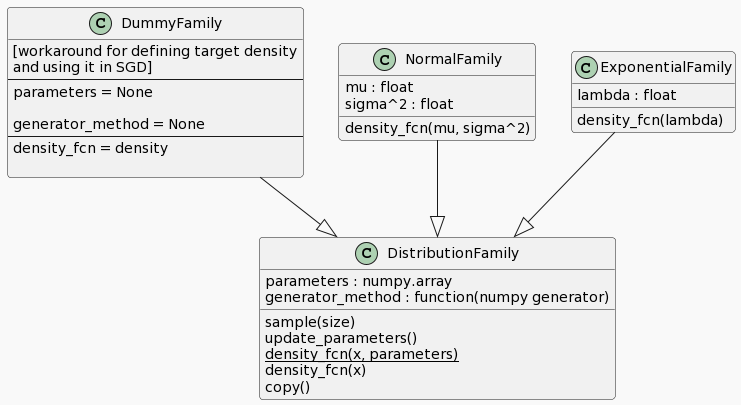
\includegraphics[width=0.95\linewidth]{Images/code/UML_distribution_family.png}

The code also allows for quick changes of other settings such as the "metrics" used to optimize the parameter of the sampling policy. As long as you can implement the Importance Sampling estimator of the gradient of the likelihood or loss function, you can just pass this estimator (which is a function) as a parameter of the wAIS estimator, and the algorithm will optimize $q_t$ using this criterion instead of having to reimplement the whole algorithm.

As a conclusion, the code was meant to be flexible, in order to approach the optimization of $q_t$ with the best accuracy possible if we have some hints on the form of that distribution. Indeed one could even perform a Gradient Descent using Kullback Leibler or Rényi's alpha-divergence with two distributions from different Families, which allows approximation.

\subsubsection{Possible improvements}

\begin{itemize}

\item Some code hasn't been factorized to its most minimal variant potential. There might be some code that can be reduced in various places. However, the code should be well factorized overall.

\item The code doesn't support yet discrete distributions because the gradient descent requires a function which is differentiable, however one could consider using finite difference in order to maybe achieve the same kind of results.

\item In order to make sure we still continue to explore the entire space even though we found a distribution which is a local minimum of the Likelihood function, we could consider space exploration tactics such as sampling from another distribution in the same family with a low probability (like 5\% and up to 10\% ). The parameter of that distribution would be determined by going from the stable current parameter and continue going in the same direction as the last gradient step taken.

\item Finally one could implement a DistributionFamily child class for mixtures of Normal Laws which could lead to interesting approximations of the target optimal density
\end{itemize}

\begin{figure}[H]
    \centering
    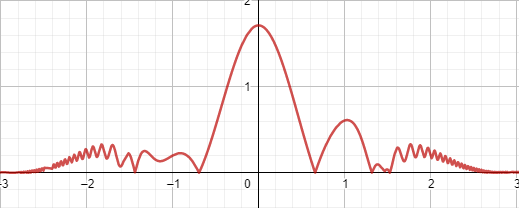
\includegraphics[width=\linewidth]{GeoGebra_cRvCokDFIT.png}
    \caption{a case of a target optimal policy for wAIS which could be hard to properly approximate using only a normal law}

    in this particular case :

    $$\varphi : x \mapsto \sin(x^5) - 3 \cos(3x)$$
    $$\pi = \phi : x \mapsto \frac{e^{- \frac {x^2}{2}}}{\sqrt{2 \pi}}$$

    function showed: target density $x \mapsto \pi(x) \left\vert \varphi(x) - I \right\vert$
    
    \label{fig:complexdistrib}
\end{figure}